\documentclass{beamer}

\usetheme{default}
\usepackage{graphicx}
\usepackage{booktabs}
\usepackage{xcolor}

% Define custom colors based on styles.css
\definecolor{imdbYellow}{HTML}{F5C518} % IMDb yellow
\definecolor{imdbBlack}{HTML}{000000} % Black background
\definecolor{imdbWhite}{HTML}{FFFFFF} % White text
\definecolor{imdbHoverYellow}{HTML}{E4B10F} % Hover yellow

% Apply the custom colors
\setbeamercolor{background canvas}{bg=imdbBlack}
\setbeamercolor{normal text}{fg=imdbWhite}
\setbeamercolor{frametitle}{bg=imdbYellow, fg=imdbBlack}
\setbeamercolor{title}{fg=imdbYellow}
\setbeamercolor{subtitle}{fg=imdbYellow}
\setbeamercolor{section in toc}{fg=imdbYellow}
\setbeamercolor{item}{fg=imdbYellow}
\setbeamercolor{block title}{bg=imdbYellow, fg=imdbBlack}
\setbeamercolor{block body}{bg=imdbBlack, fg=imdbWhite}

% Set font for better readability
\usepackage{lmodern}
\renewcommand{\familydefault}{\sfdefault}

\title[HistFlix: Resultados e Web App]{HistFlix: Resultados, Desempenho e Demonstração da Aplicação Web}
\author{Bruno Baltuilhe, Isaque Pimentel, Kelly Graziely Pena}
\institute{Universidade Presbiteriana Mackenzie}
\date{Aula 4 -- Junho/2025}

\begin{document}

% Slide de Título
% Roteiro: Olá, somos o grupo responsável pelo HistFlix, um sistema de recomendação personalizado para filmes históricos. Vamos apresentar os resultados, desempenho e uma demonstração da aplicação web.
\begin{frame}
    \titlepage
\end{frame}

% Slide 1: Resumo do Projeto
% Roteiro: O objetivo do HistFlix é recomendar filmes e documentários históricos de forma personalizada, combinando técnicas de filtragem colaborativa, baseada em conteúdo e análise de sentimentos. A interface é bilíngue e amigável, com foco em engajamento educacional.
\begin{frame}{Resumo do Projeto}
    \textbf{HistFlix:} Sistema de recomendação híbrido para filmes e documentários históricos.
    \vspace{0.5cm}
    \begin{itemize}
        \item Combina filtragem colaborativa, baseada em conteúdo e análise de sentimentos.
        \item Interface web bilíngue e amigável.
        \item Foco em personalização e engajamento educacional.
    \end{itemize}
\end{frame}

% Slide 2: Arquitetura Final do Sistema 1/2
% Roteiro: O fluxo de dados começa com a extração e pré-processamento do MovieLens. Os dados alimentam dois módulos principais: o híbrido, que combina SVD e similaridade de conteúdo, e o de análise de sentimentos, que interpreta emoções do usuário e as mapeia para gêneros. Toda a lógica é integrada em uma aplicação web modular usando Flask.
\begin{frame}{Arquitetura Final do Sistema 1/2}
    \textbf{Principais Componentes:}
    \begin{itemize}
        \item Extração e pré-processamento de dados (MovieLens).
        \item Modelos de recomendação híbrida (SVD + matriz de similaridade do cosseno) 
        \item Análise de sentimento (TextBlob + VADER): mapping sentimentos para generos.
        \item Aplicação web modular (usando Flask).
    \end{itemize}
\end{frame}

% Slide 2: Arquitetura Final do Sistema 2/2
% Roteiro: Aqui vemos a interface inicial da aplicação, onde o usuário pode escolher entre recomendação híbrida ou por sentimento, além de alternar o idioma.
\begin{frame}{Arquitetura Final do Sistema 2/2}
    \begin{center}
        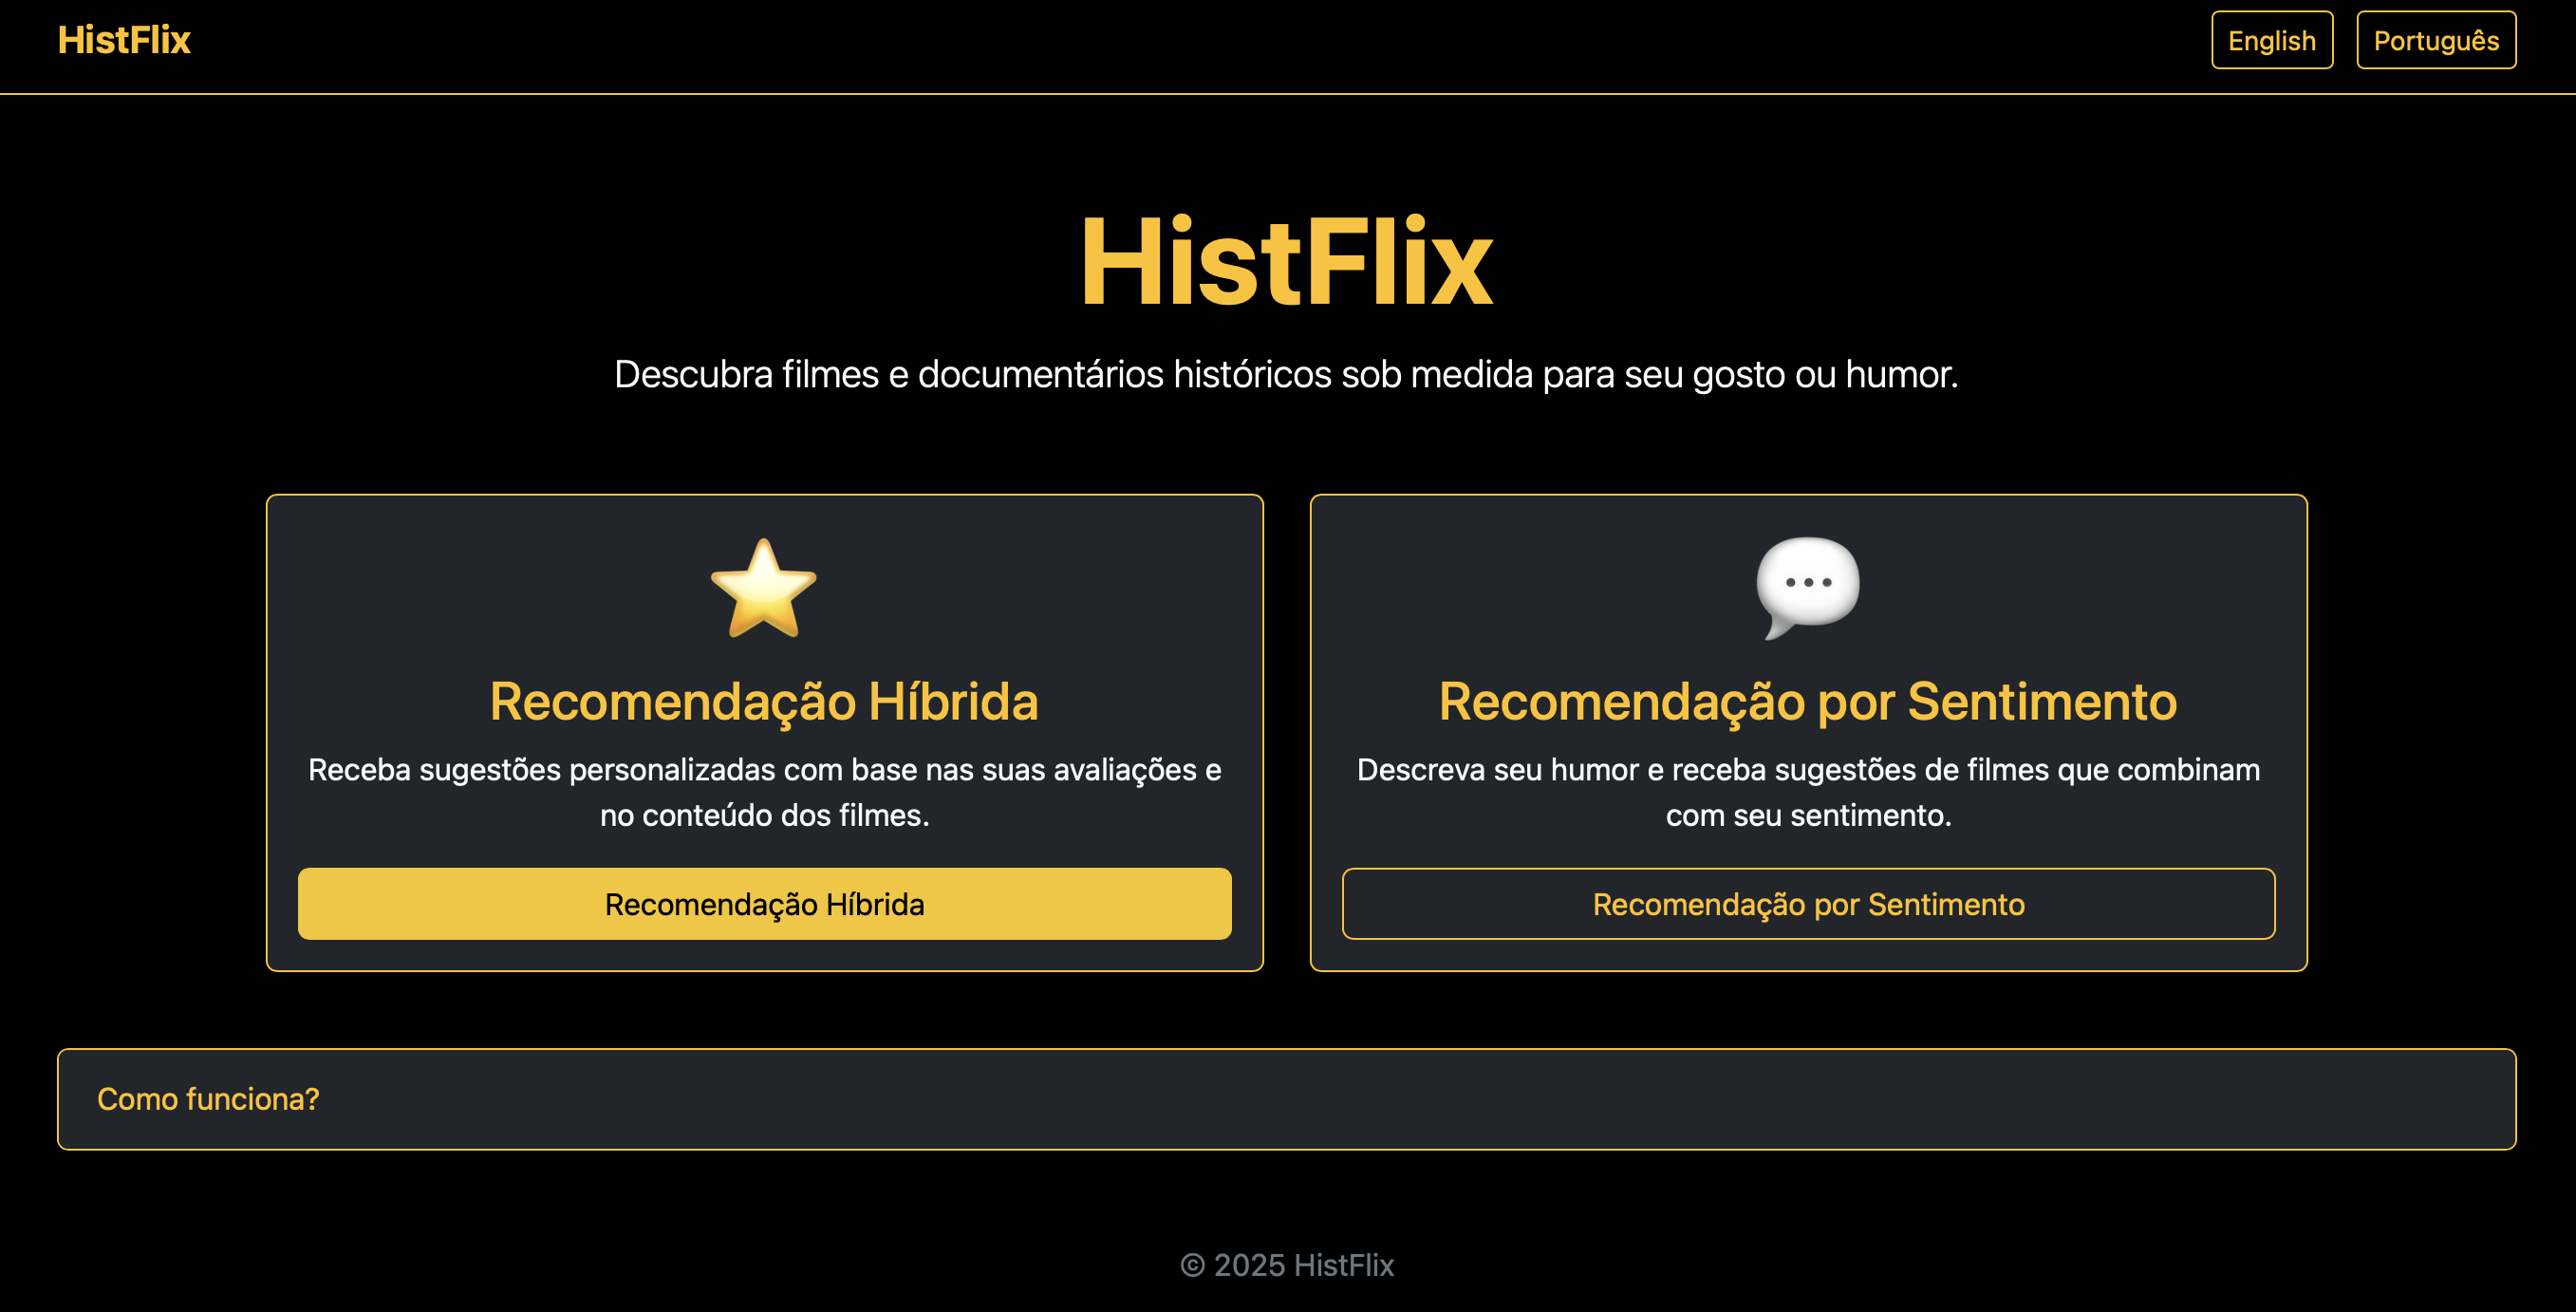
\includegraphics[width=0.95\textwidth]{../pictures/home_page.png}
    \end{center}
\end{frame}

% Slide 3: Resultados Quantitativos
% Roteiro: Avaliamos o desempenho dos modelos com e sem recency. O modelo sem recency apresentou maior precisão e recall, enquanto o com recency prioriza tendências recentes, mas reduz a novidade. Ambos mantêm alta diversidade.
\begin{frame}{Resultados Quantitativos}
    \textbf{Desempenho dos Modelos (MovieLens 1M):}
    \vspace{0.3cm}
    \begin{tabular}{lcccccc}
        \toprule
        \textbf{Modelo} & \textbf{RMSE} & \textbf{Prec@10} & \textbf{Rec@10} & \textbf{Cobertura} & \textbf{Diversidade} & \textbf{Novelty} \\
        \midrule
        Com Recency & 0.89 & 0.65 & 0.02 & 0.07 & 1.00 & 838.7 \\
        Sem Recency & 0.93 & 0.81 & 0.32 & 0.17 & 1.00 & 881.2 \\
        \bottomrule
    \end{tabular}
    \vspace{0.3cm}
    \begin{itemize}
        \item \textbf{Interpretação:} Modelo sem recency tem maior precisão e recall, mas menor novidade.
    \end{itemize}
\end{frame}

% Slide 5: Demonstração da Aplicação Web
% Roteiro: A aplicação permite recomendações híbridas e por sentimento, com interface bilíngue, navegação intuitiva e mensagens de erro explicativas. O usuário pode receber sugestões alinhadas ao seu perfil ou ao seu estado emocional.
\begin{frame}{Demonstração da Aplicação Web}
    \textbf{Principais Funcionalidades:}
    \begin{itemize}
        \item Recomendação híbrida e por sentimento.
        \item Interface bilíngue (PT/EN), navegação intuitiva.
        \item Mensagens de erro amigáveis e explicações das recomendações.
    \end{itemize}
    \vspace{0.3cm}
    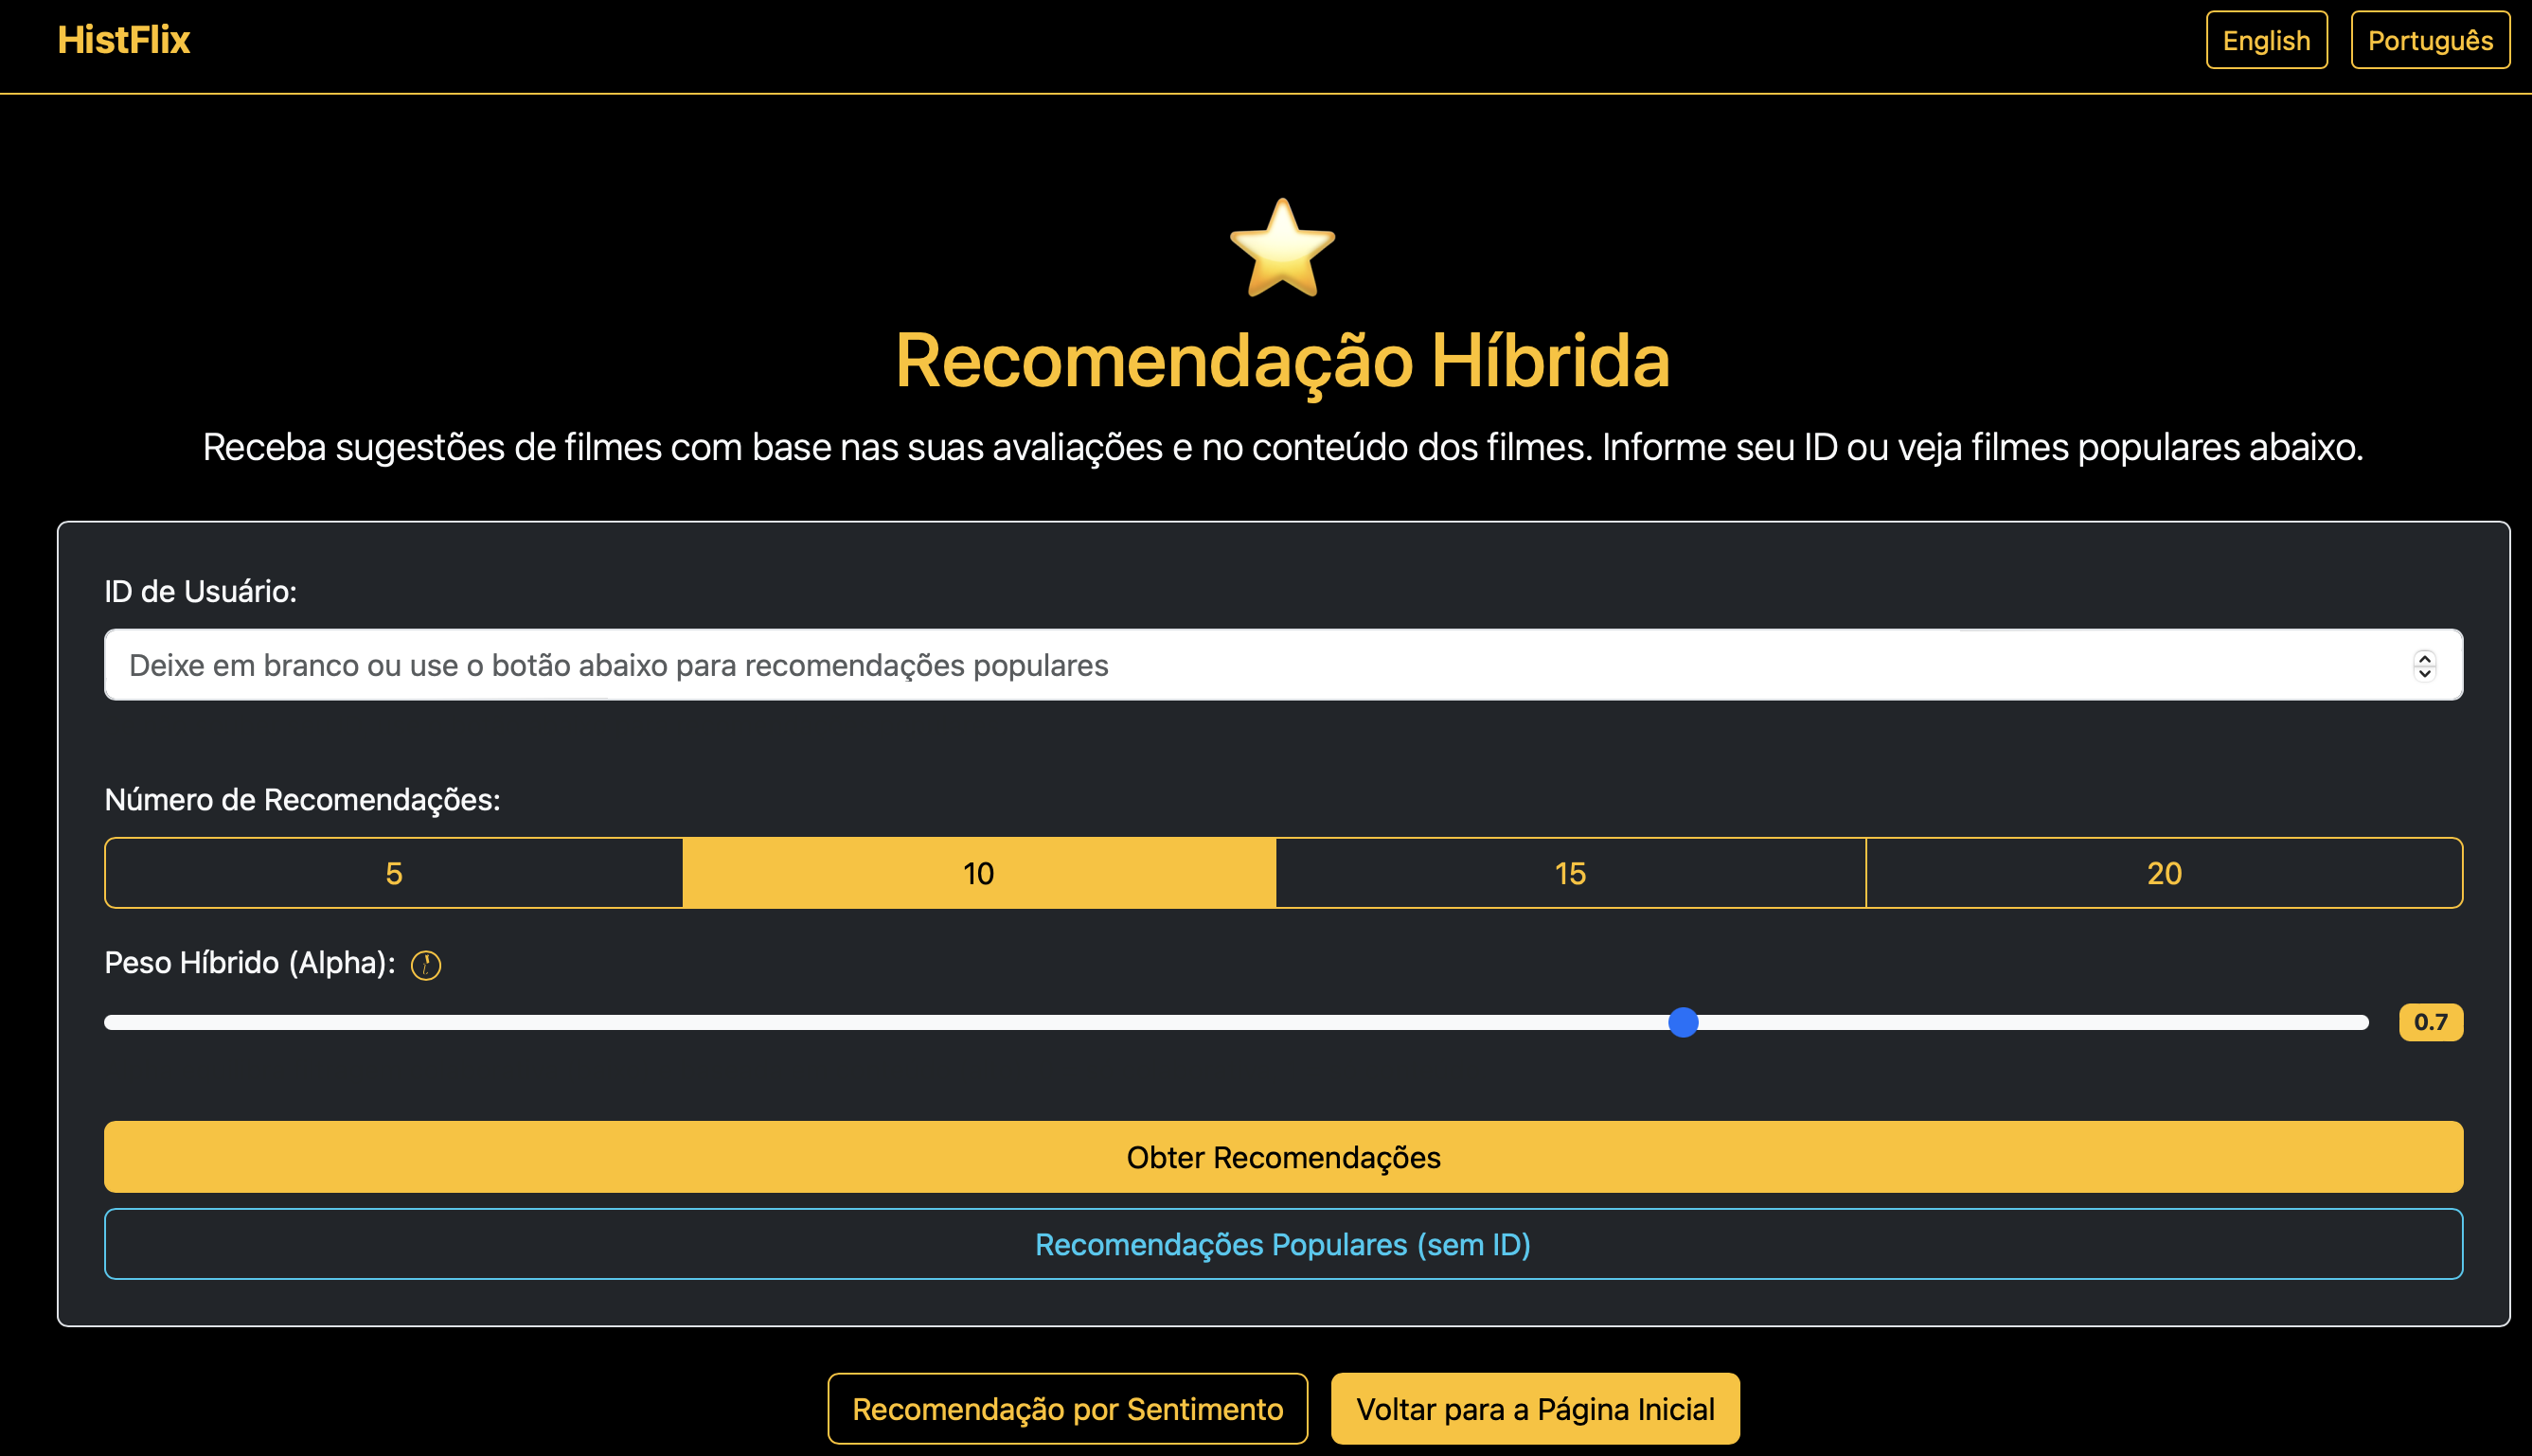
\includegraphics[width=0.45\textwidth]{../pictures/hybrid_recommendation.png}
    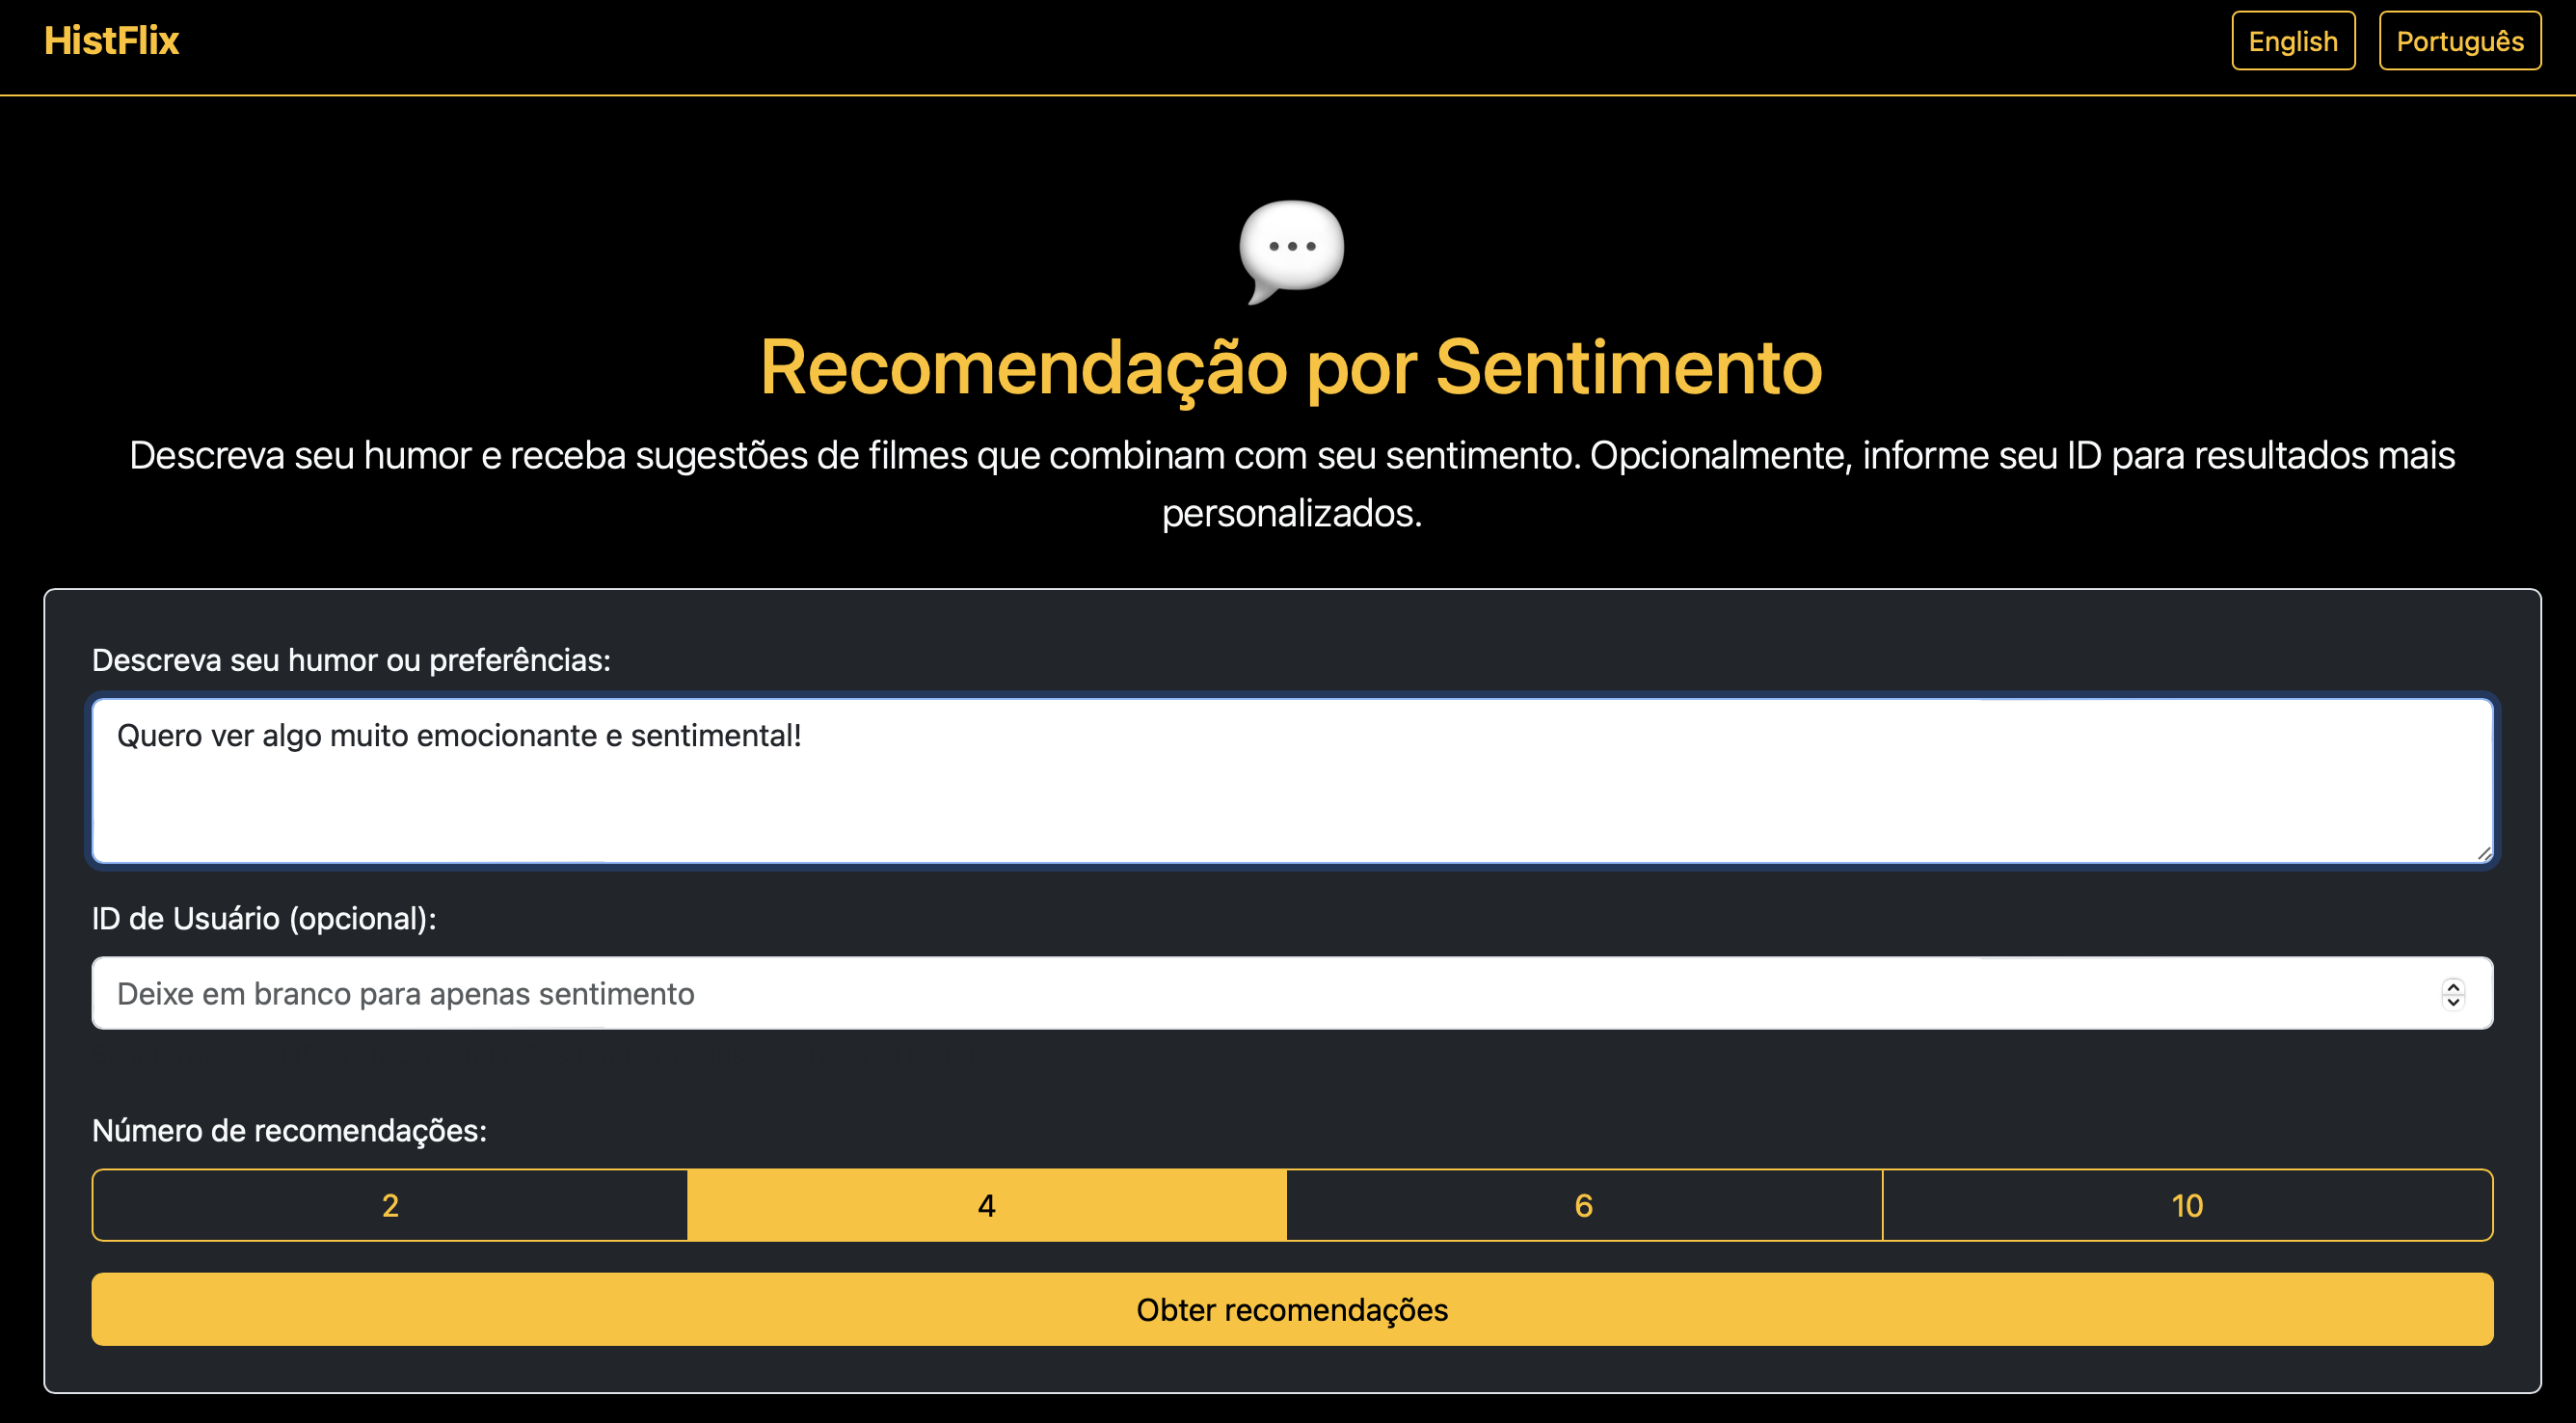
\includegraphics[width=0.45\textwidth]{../pictures/sentiment_recommendation.png}
\end{frame}

% Slide 6: Pontos Positivos e Negativos
% Roteiro: Entre os pontos positivos, destacamos a arquitetura modular, resultados competitivos e interface clara. Como desafios, ainda há o problema do cold start, dependência de avaliações e espaço para expandir a análise de sentimentos.
\begin{frame}{Pontos Positivos e Negativos}
    \textbf{Pontos Positivos:}
    \begin{itemize}
        \item Arquitetura modular e código reutilizável.
        \item Resultados competitivos nas métricas de recomendação.
        \item Interface clara e suporte bilíngue.
    \end{itemize}
    \vspace{0.3cm}
    \textbf{Pontos a Melhorar:}
    \begin{itemize}
        \item Cold start para novos usuários/filmes.
        \item Dependência de dados de avaliações.
        \item Possibilidade de expandir análise de sentimentos.
    \end{itemize}
\end{frame}

% Slide 7: Melhorias Futuras
% Roteiro: Para o futuro, pretendemos incorporar modelos de PLN mais avançados, ampliar a base de dados, criar uma versão mobile e aprofundar a personalização das recomendações.
\begin{frame}{Melhorias Futuras}
    \begin{itemize}
        \item Incorporar modelos de PLN mais avançados (ex: BERT).
        \item Ampliar base de dados (ex: MovieLens 32M).
        \item Desenvolver versão mobile e recomendações em tempo real.
        \item Personalização mais profunda por perfil e contexto.
    \end{itemize}
\end{frame}

% Slide 8: Conclusão e Agradecimentos
% Roteiro: O HistFlix se mostrou robusto e promissor para recomendações históricas personalizadas. Obrigado pela atenção! Fiquem à vontade para testar a aplicação ou entrar em contato.
\begin{frame}{Conclusão e Agradecimentos}
    \textbf{HistFlix:} Sistema robusto, modular e com resultados promissores para recomendações históricas personalizadas.
    \vspace{0.5cm}
    \textbf{Obrigado!}
    \vspace{0.5cm}
    \begin{itemize}
        \item Dúvidas? Teste a aplicação ou entre em contato!
    \end{itemize}
\end{frame}

\end{document}
